\documentclass{article}
\usepackage[paperheight=10.75in,paperwidth=9.5in,margin=.2in]{geometry}
\usepackage[sfdefault]{roboto}
\usepackage[T1]{fontenc}
\usepackage{graphicx}

\begin{document}
\pagenumbering{gobble}

\begin{samepage}
\noindent \textbf{Supplemental Figure S3.}
Densities of the top three enriched motifs at ends of chromosomal \textit{q} arms of datasets
\textbf{(A)} HG001,
\textbf{(B)} HG003,
\textbf{(C)} HG004,
\textbf{(D)} HG005,
\textbf{(E)} HG006, and
\textbf{(F)} HG007.
Only the arms covered by at least 25 reads across all datasets are displayed.
Genomic coordinates are given in kbp.
Vertical red dashed lines denote the position of the boundary of the annotated telomeric tract.

\begin{figure}[ht!] \centering
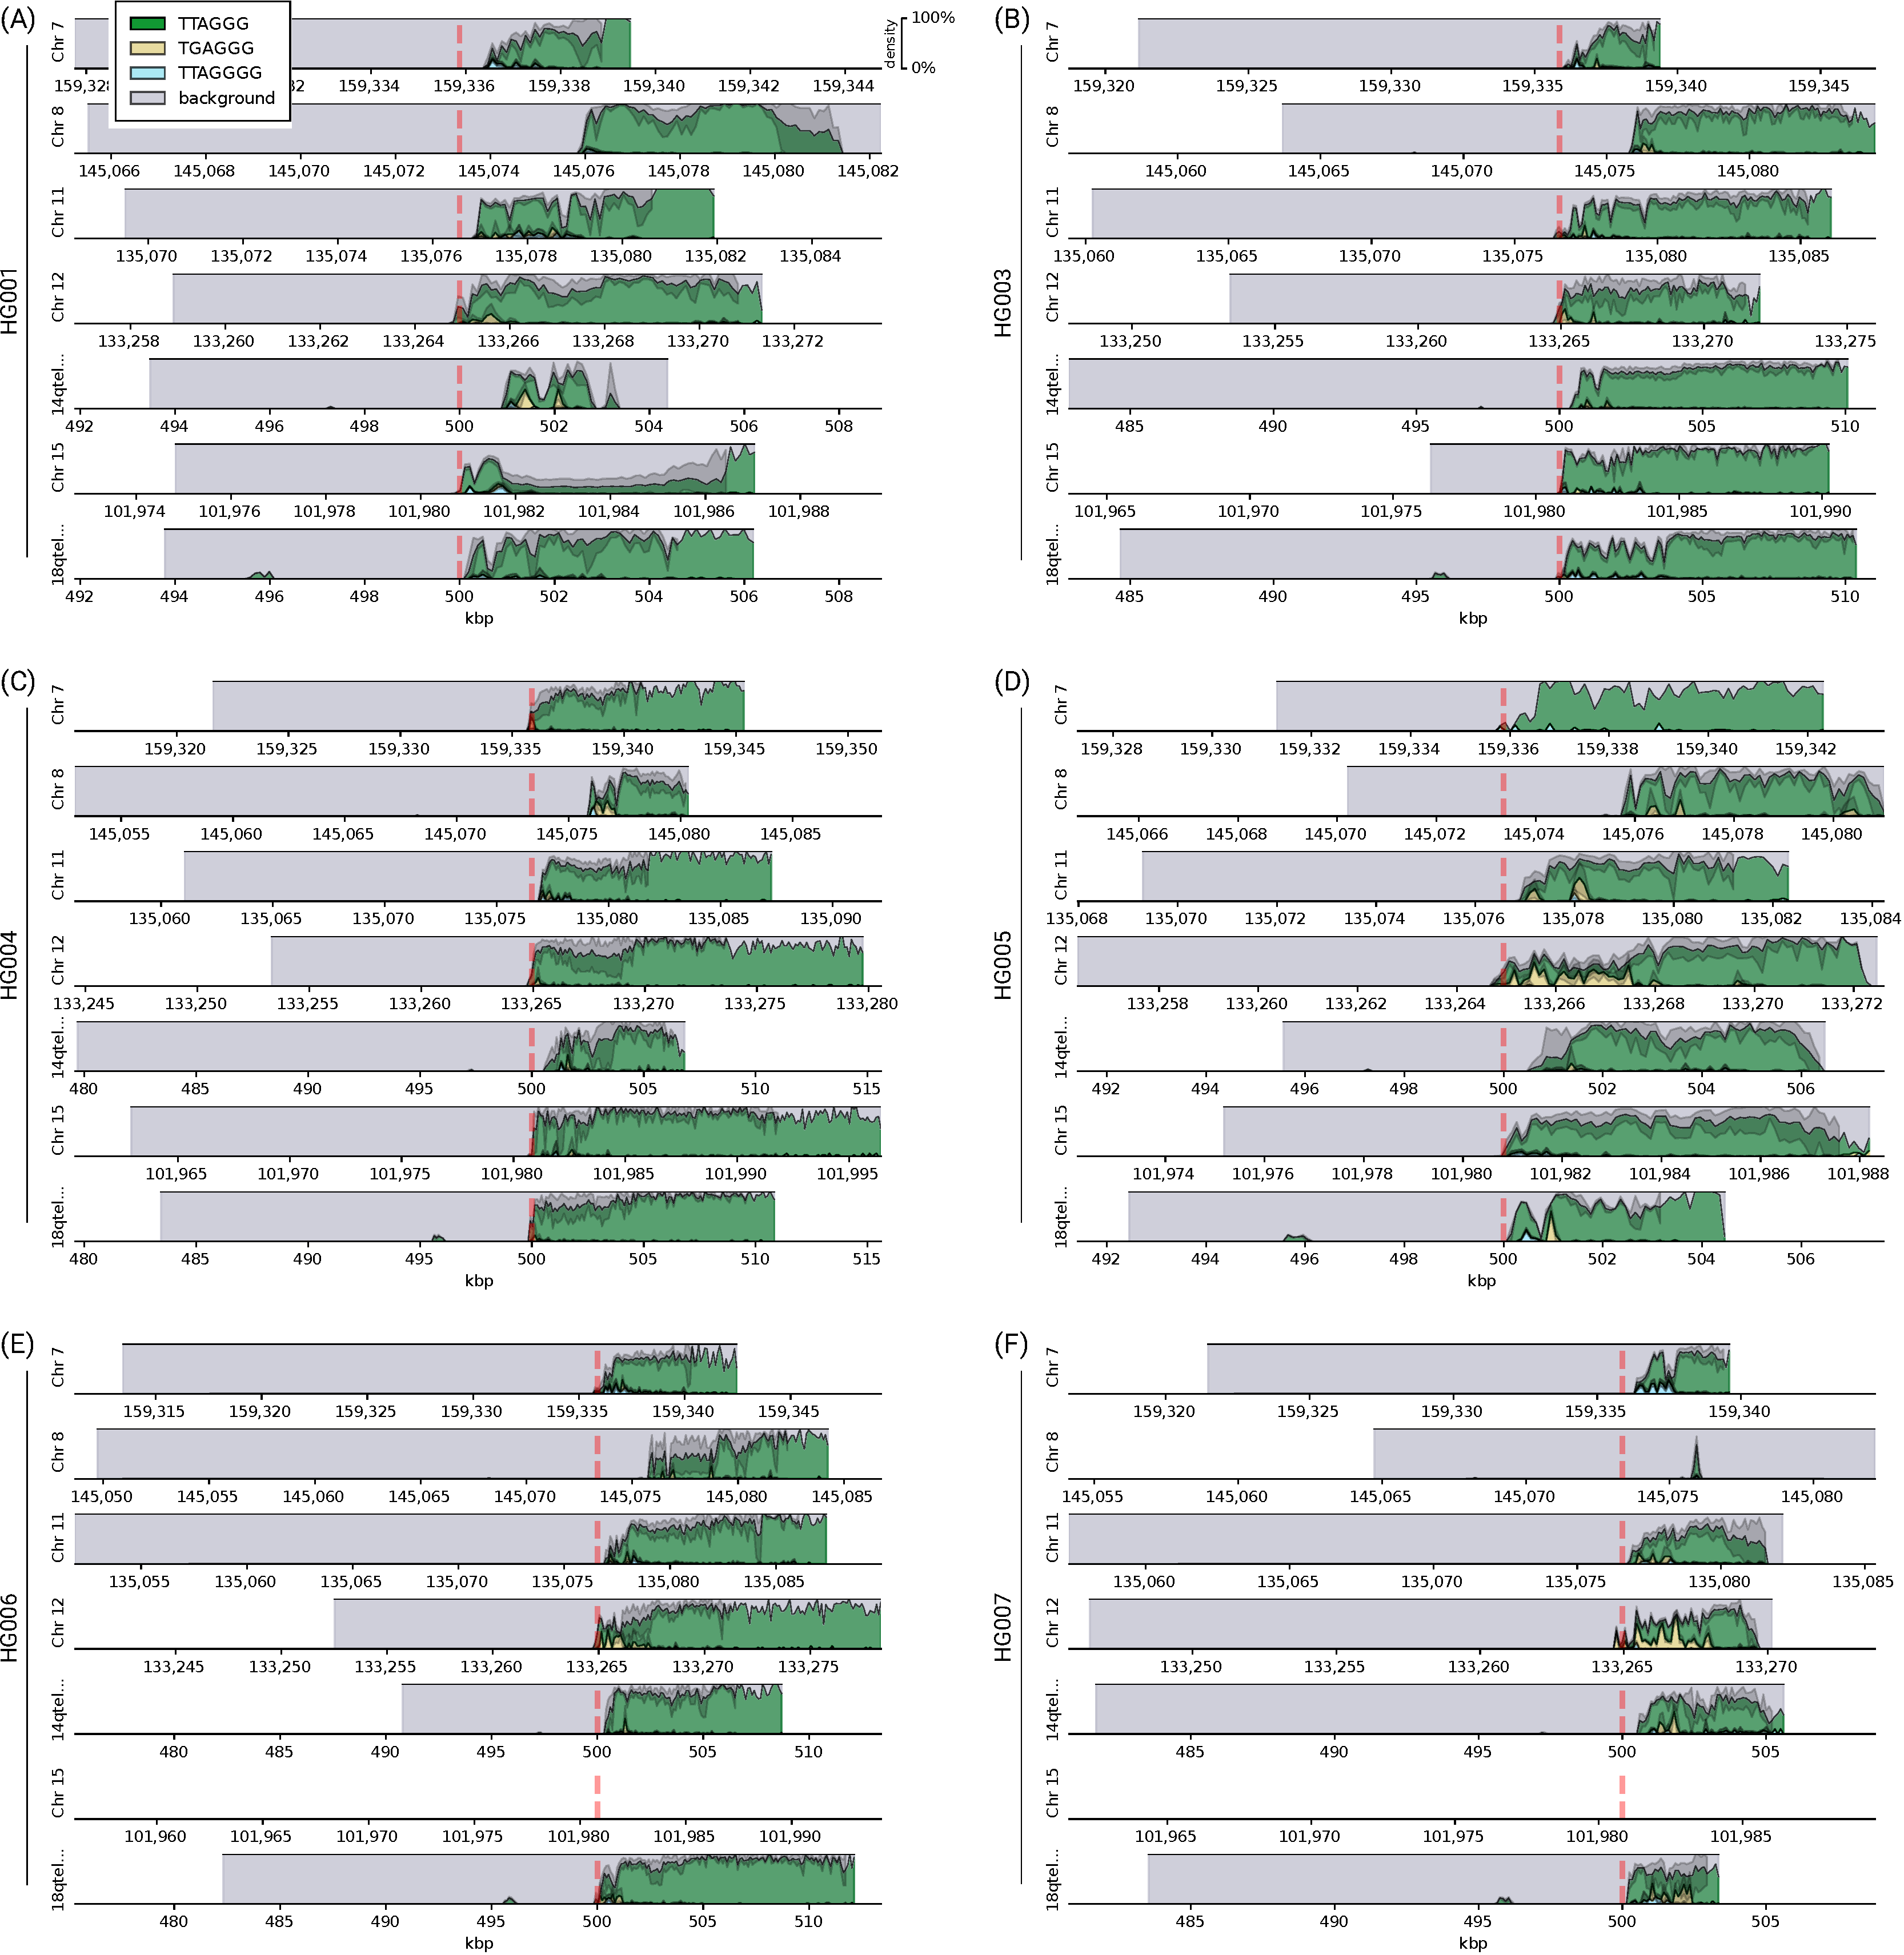
\includegraphics[width=\textwidth,keepaspectratio]{Figure_S3-nolegend.pdf}
\end{figure}
\end{samepage}

\end{document}
